\documentclass[a4paper]{article}
\usepackage[utf8]{inputenc}
\usepackage{graphicx}
\usepackage{twocolpceurws}
\usepackage{xcolor}
\usepackage{url}

\def\infinity{\rotatebox{90}{8}}


\title{Damegender: Towards an International and Free Dataset about Name, Gender and Frequency}

\author{
David Arroyo Menéndez, Jesus González-Barahona, Gregorio Robles \\ Grupo de Sistemas y Comunicaciones (GSyC) \\ Universidad Rey Juan Carlos, Madrid, Spain \\ \{d.arroyome@alumnos, jgb@gsyc, grex@gsyc\}.urjc.es
}


\newif\ifdraft
\drafttrue
%\draftfalse
\newcommand{\nb}[2]{
	{
		{\color{black}{
				\small\fbox{\bfseries\sffamily\scriptsize#1}
				{\sffamily\small$\triangleright~${\it\sffamily\small #2}$~\triangleleft$}
	}}}
}


\ifdraft
\newcommand\davidam[1]{\nb{David}{\color{olive}#1}}
\newcommand\grex[1]{\nb{Gregorio}{\color{red}#1}}
\newcommand\jgb[1]{\nb{Jesús{\color{blue}#1}}}
\newcommand\fixme[1]{{\textcolor{red}{[FIXME] #1}}}
\newcommand\cn{{\color{violet}[citation required]}}

\else
\usepackage[disable]{todonotes}
\newcommand\gema[1]{}
\newcommand\grex[1]{}
\newcommand\mei[1]{}
\newcommand\fixme[1]{}
\newcommand\cn{}


\fi
\let\labelindent\relax
\usepackage[inline]{enumitem}





\institution{}


\begin{document}

\maketitle

\begin{abstract}
  %% Introduction

  Equality of gender is the 5th objective of sustanaible development
  in United
  Nations\footnote{https://www.un.org/sustainabledevelopment/gender-equality/}.

  This equality can be reached working on measure and analyze data and
  to apply politics from the results. On many gender studies, we need
  to count males and females deciding gender from names, for instance,
  research papers, job positions, streets, ... The traditional way is
  to use commercial APIs with propietary data without idea about how
  the data has been built. Another way, is taking data from wikipedia
  or scientific sites.

  %% Methodology

  With Open Data idea, many statistics institutions are providing Open
  Datasets about name, gender and frequency. So, we need a scientific
  discussion about unifying formats, make easy ways to process these
  data and ways towards make standards. In this discussion, we take
  into account minorities, for example, LGTB claims such as attending
  the non binary reality.

  %% Results
  
  The dataset is covering more than 20 countries in the occidental
  world. Having more names than any open source software in this
  moment. Allowing to measure gender gap to students and academics
  interested on the phenomenon.

  %% Conclusion

  There are a warranty of quality on reproducible research the
  citation about official sources provided by statistics institutions
  making easy the peer review and opening doors to the semantic web
  and the attention to minorities such as trans gender people, or
  cultures with own languages in states with another main language
  doing more cheaper to measure the gender gap.
  
\end{abstract}


\section{Introduction}

In recent times, many research investigations have been made on gender diversity in the IT domain.
Examples of these efforts range from the participation in Twitter~\cite{burger2011discriminating,mislove2011understanding},
in Wikipedia~\cite{antin2011gender,hill2013wikipedia}, in science~\cite{holman2018gender,dollar1999gender}, and more specifically in the software domain in StackOverflow~\cite{vasilescu2012gender,vasilescu2015gender}, GitHub~\cite{vasilescu2015gender}, and free software development~\cite{robles2014floss,izquierdo2018openstack,lee2019floss,catolino2019gender}.

The interest on gender diversity has become more and more relevant, and so does the identification methods that allow us to perform comprehensive studies on gender representation, given the large amounts of data available, in particular from collaborative environments.

The most used method to infer the gender of participants is by looking at their name.
However, there are some studies about Twitter and GitHub where not only names are used to detect gender. 
In those studies we can find gender detection tools that infer the gender from faces in images~\cite{ranjan2017hyperface}, from hand-written annotations~\cite{liwicki2011automatic}, or from speeches~\cite{koppel2002automatically}.

Currently, there are different ways to detect gender from a person's name (and maybe other personal data, such as the surname, the geographic location, etc.).
A first one is based on data extracted from the Wikipedia, self-references in trust websites, searches in Google Images, among others.
Another way to do it is by using one of the existing Application Programming Interfaces (APIs).
This paper is about the latter, focusing on their possibilities and limitations.
Therefore, (i) we evaluate the quality (and accessibility, including price) of different existing solutions;
(ii) we discuss their limitations; and
(iii) we investigate what happens with those names not included in a census, for example, nicknames or diminutives.
% and (iv) we elaborate on how massive gender detection from Internet, for example, mailing lists or software repositories, can be done.

As a result, we contribute with: 
(i) an evaluation of the quality of different solutions applying well-known metrics;

(ii) a tool, called \texttt{damegender}, guessing gender from a name
  giving support to Spanish and English from the open data census
  provides by the states built to understand current technologies in
  detail; this tool has been compared with APIs using an international
  dataset with good results; and
  
(iii) a machine learning solution to strings not found in the census
  dataset to approach the problem with nicknames and diminutives;
  
%(iv) a proof-of-concept of \texttt{damegender} to detect gender in mailing lists and software repositories.

%A summary of current features of \texttt{damegender} are:
%
%\begin{itemize}
% \item To deduce the gender about a name in Spanish or English (current status) from open census in local.
% \item To decide about males and females in strings using different machine learning algorithms.
% \item To use the main solutions in gender detection (genderize, genderapi, namsor, nameapi and gender guesser) from a command.
% \item To allow research to link names to males or females, based on statistical . We provide Python commands to study and compare gender solutions with confusion matrix, accuracies, and error measures. And to decide about features: statistical feature weight, principal component analysis, ...
% \item To determine gender gap in free software repositories or mailing lists (proof of concept).
%\end{itemize}

The remainder of this paper is structured as follows:

In Section~\ref{sec:truehood} we discuss the different ways to find
evidence about names, gender and frequency.

Section~\ref{sec:diversity} introduces the diversity discussion about
minorities (cultural, LGTB, ...)

Section~\ref{sec:semantic} is giving clues about how to approach the
semantic web goals with the previous dicussion presented.

Section~\ref{sec:damegender} reports on values of accuracy and offers
a confusion matrix using a scientific dataset.

Section~\ref{sec:measuring} is about how we use Machine Learning in
\texttt{damegender}.  Section~\ref{sec:datasets} discusses limitations
and further research, and concludes the paper.

\section{Truehood and Falsehood in names, gender and frequency}
\label{sec:truehood}

The current idea in the field is the data about name, gender and
frequency is ok because there are people who is paying by it, or many
people is downloading a product. This intuition is right generally,
although sometimes the people is paying by a bad product due to a good
marketing strategy, a monopoly or there are a fraud, ... Another idea
is the people trust in the goverment about statistics such as economy,
demography, democracy, ... So the people can trust on names, gender
and frequency. In Damegender, we are trusting in both notions about
truehood: the market's point of view and the official statistics's
point of view.

Sometimes there are problems downloading the official statistics but
there are people who has retrieved these data, for example, with
webscraping. We want classify these files with another idea about
truehood.

Another problem arises when the goverment does little chances in the
data, sometimes communicating it to the users and another times
not. That could be a problem about upgrades, but it's not a problem
with the truehood, although it's possible make a trace about this
chances.

Another sources to retrieve gender and names can be personal
scientific websites, wikipedia, or similar, but these sources is not
giving the frequency, now. So, we are rejecting this idea. 

With an international free dataset about names, gender and frequency
we can build reproducible science in fields such as Natural Language
Processing (gender detection from the name), social sciences (gender
gap~\cite{holman2018gender,mislove2011understanding}),
lingüistic~\cite{lawson2005russian,krueger1962mongolian,van2020gender},
software engineering~\cite{vasilescu2012gender}, ...

%% CITAR okal2018linguistic


\section{Gender, Language, Nation and Diversity}
\label{sec:diversity}

The first intuition about gender is male or female, but there non
binary options about gender such as transgender that is changing laws
in the goverments, so in some states a person can be registered as non
male and non female. There are Open Datasets not provided by states
about names classified as transgender. A good option is to wait the
updates in laws and releases in open datasets with these non binary
ideas. Meanwhile, it's possible to give to the users software to
understand how many males and females is using a name.

Exists rules and exceptions in the languages to predict if a name is
about male or female when you don't know the name. For example, in
spanish or english there are more names ending with 'a' classified as
females than classified as males. And Andrea is female in Spain and
male in Italy. So, it's useful to understand the language and culture
associated with a name. Language is close to nation, but there are
differences, for example, in Spain there are several languages basque,
catalan, castillian, ... or the spanish is the main language in Spain
and in another countries such as Argentina, Mexico, Ecuador, Bolivia,
... So, it would be useful to detect the language and nation from
names and surnames to help to detect gender.

Some countries, such as Spain, are providing free datasets about
surnames but we need more efforts from many countries on this
objective. On other hand, there are previous works to relate name and
surnames with ethnicity using Wikipedia and Machine Learning.
%% ************ Citar **********
%% Name-Ethnicity Classification from Open Sources


\section{Semantic Web}
\label{sec:semantic}

When we are describing people with names and gender could be giving
semantic richness with semantic markup taking into account the lessons
learned about the domain, for example, using microformats. Changing the
current situation using a poor html:

\begin{verbatim}
<table class="infobox" style="width:22.7em; 
line-height: 1.4em; text-align:left; 
padding:.23em;">
  <tbody>
    <tr><th colspan="3" class="cabecera"
style="text-align:center;color:black;">
           Juan</th></tr><tr>
[...]
<tr><th scope="row"
style="text-align:left">
<a href="/wiki/Identidad_sexual" 
   title="Identidad sexual">Género</a>
</th><td colspan="2"> Masculino</td></tr>
\end{verbatim}

Towards the semantic way:

\begin{verbatim}
<div class="h-card">
  <span class="p-name">Emma Goldman</span>
  <span class="p-gender p-gender-female 
               p-gender-female-us 
               p-gender-female-inter">
         Female
  </span>      
  <span class="p-street-address">
         123 Main St
  </span>
  <span class="p-locality">Some Town</span>
  <span class="p-region">CA</span>
  <span class="p-postal-code">90210</span>
</div>
\end{verbatim}

With a richness markup take into account the gender in the context of
a country.

\section{Damegender Open Datasets Collection}
\label{sec:damegender}

In Damegender, we have unified the different formats to name, gender
and frequency from official sources in these countries: Austria,
Australia, Belgium, Canada, Denmark, Germany, Spain, Finland, France,
Great Britain, Ireland, Mexico, New Zealand, Portugal and Slovenia.

Later, we have merged these datasets building a free and international
dataset.

Generally, these data are providing name, gender and frequency about
births (Canada), although in some countries (Spain) are giving the
total.

We have found open datasets about countries such as Turkey and China
retrieved by another open source developers that is being included in
Damegender, but not in the international dataset. In Turkey the data
has been retrieved using webscraping. And in China the data has been
built by a company in collaboration with the China goverment and
contributed to R language program. We want compare precision about
this dataset with the commercial solutions to understand the truehood
about these datasets.

When the work is finished, we could to rebuild machine learning models
to predict new names and nicknames in any language and culture.

\section{Measuring Gender Gap. GNU/Linux as Use Case}
\label{sec:measuring}

With a trust open dataset about names, gender and frequency is too
easy to measure gender gap. Doing cheap to measure gender gap more
students and academic people could work in the fith Objective
Development Sustainaible of United Nations: to delete the gender gap.

This section is divided counting males and females in Debian, GNU and
Linux.

We have reached the csv files from different ways to know the names
about the people in these communities.

When this paper was being wrote in the Debian community all members
must be collaborating with a gpg key, so we can count males and females
from the keyring. The keyring was imported with gpg commands and later
was dumped the keyring in a csv file.

In the moment to write this paper
GNU\footnote{https://www.gnu.org/people/} and
Linux\footnote{https://www.kernel.org/doc/html/latest/process/maintainers.html}
has websites with the people collaborating in these projects. So,
making webscraping scripts we have downloaded the people and processed
the people to csv files

In Damegender, we have developed csv2gender, a software with a csv
file as input and deploy a statistics graph and/or return the result
of males, females and unknows about the input.

To make easy to reproduce the experiment we are pasting the commands
used with the version 0.3.4 of damegender.

\begin{verbatim}
python3 csv2gender.py files/gnu-maintainers.csv
 --first_name_position=0 
 --title="GNU maintainers grouped by gender"
 --dataset="inter" 
 --outcsv="files/gnu-maintainers.gender.csv"
 --outimg="files/gnu-maintainers.gender.png" 
 --noshow --delete_duplicated

python3 csv2gender.py files/linux-maintainers.csv
 --first_name_position=0 
 --title="Linux maintaners grouped by gender"
 --dataset="inter" 
 --outcsv="files/linux-maintainers.gender.csv"
 --outimg="files/linux-maintainers.gender.png" 
 --noshow --delete_duplicated

python3 csv2gender.py files/debian-maintainers.csv
 --first_name_position=0 
 --title="Debian maintaners grouped by gender"
 --dataset="inter" 
 --outcsv="files/debian-maintainers.gender.csv"
 --outimg="files/debian-maintainers.gender.png" 
 --noshow --delete_duplicated
\end{verbatim}

The inter dataset was created merging several open datasets downloaded
from official statistics sites from different nations: Austria,
Australia, Belgium, Canada, Germany, Denmark, Spain, Finland, Ireland,
Iceland, Mexico, New Zealand, Portugal, Slovenia, United States of
America, Uruguay and France. That's a good representation of the
Western World and the Free Software world is populating this world's
area
%% CITATION
%% ~\cite{gonzalez2008geographic}.

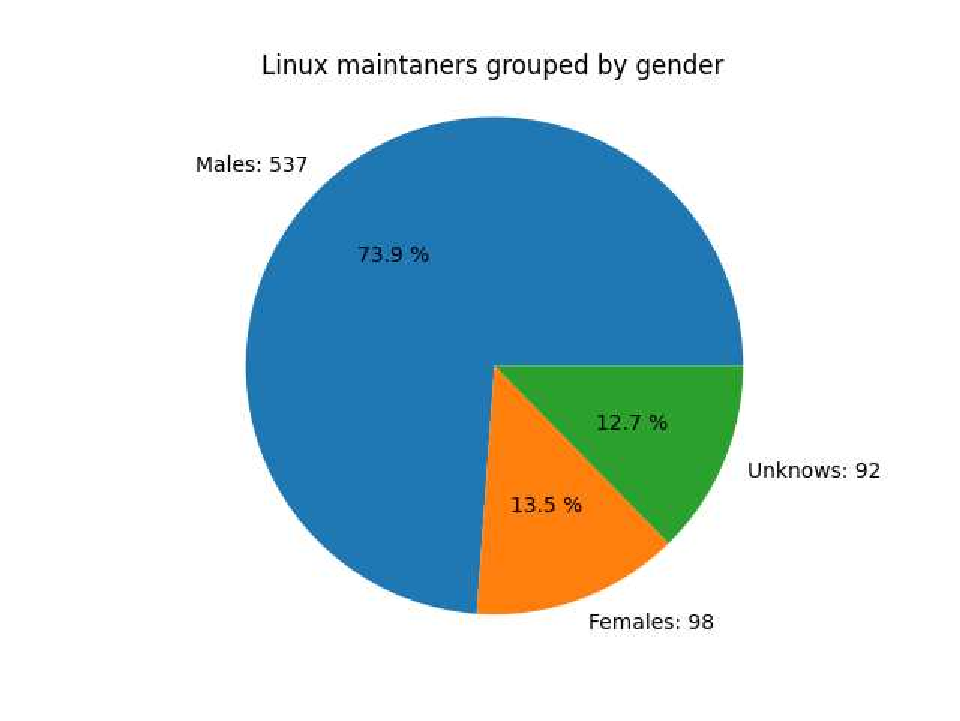
\includegraphics[height=0.4\textheight]{images/linux-maintainers.gender.pdf}

Linux divides the developers in 537 males (73.9\%), 98 females
(13.5\%) and 92 unknows (12.7\%). The number of unknows is due to
different reasons, but it's so common in Linux that the developer is a
company and not a name of a person.

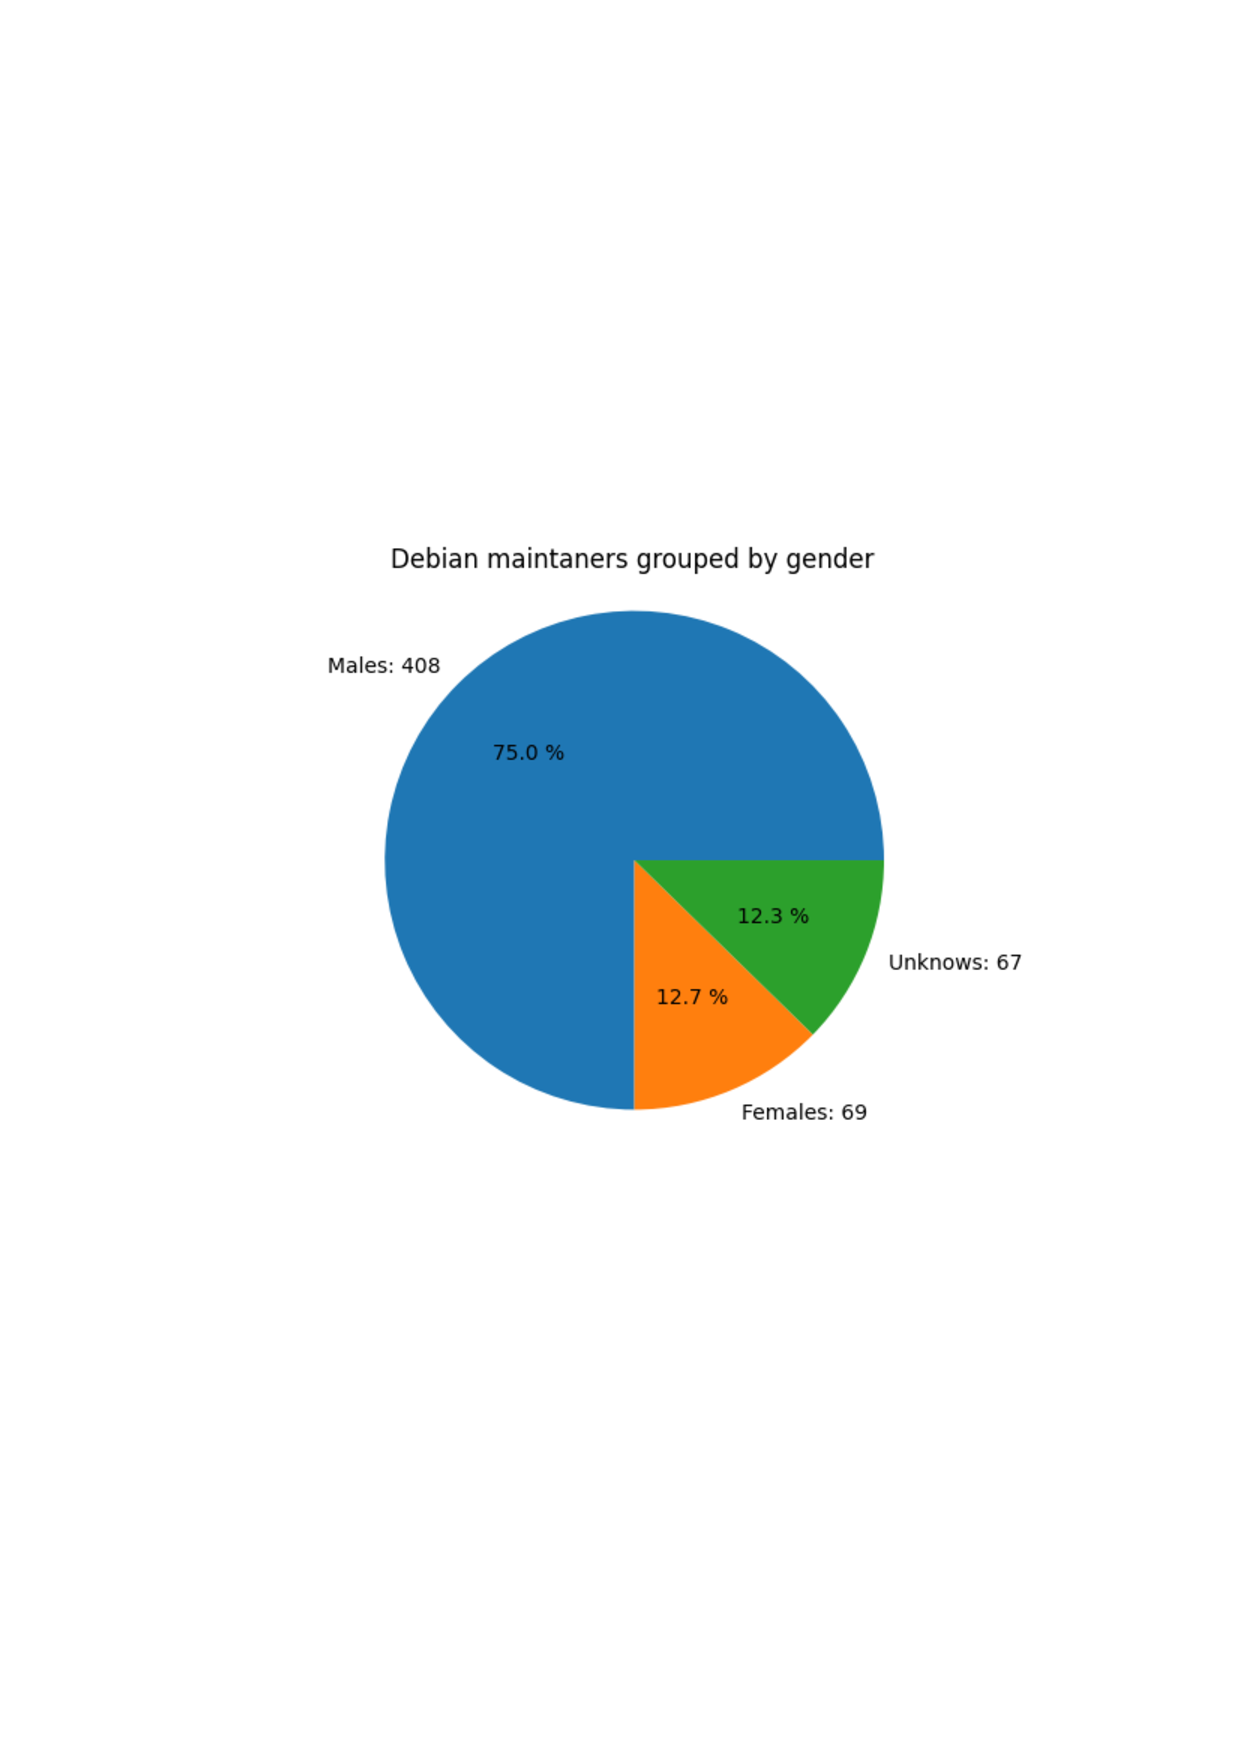
\includegraphics[width=0.6\textwidth]{images/debian-maintainers.gender.pdf}

Debian divides the developers in 408 males (75\%), 69 females (12.7\%)
and 67 unknows (12.3\%).

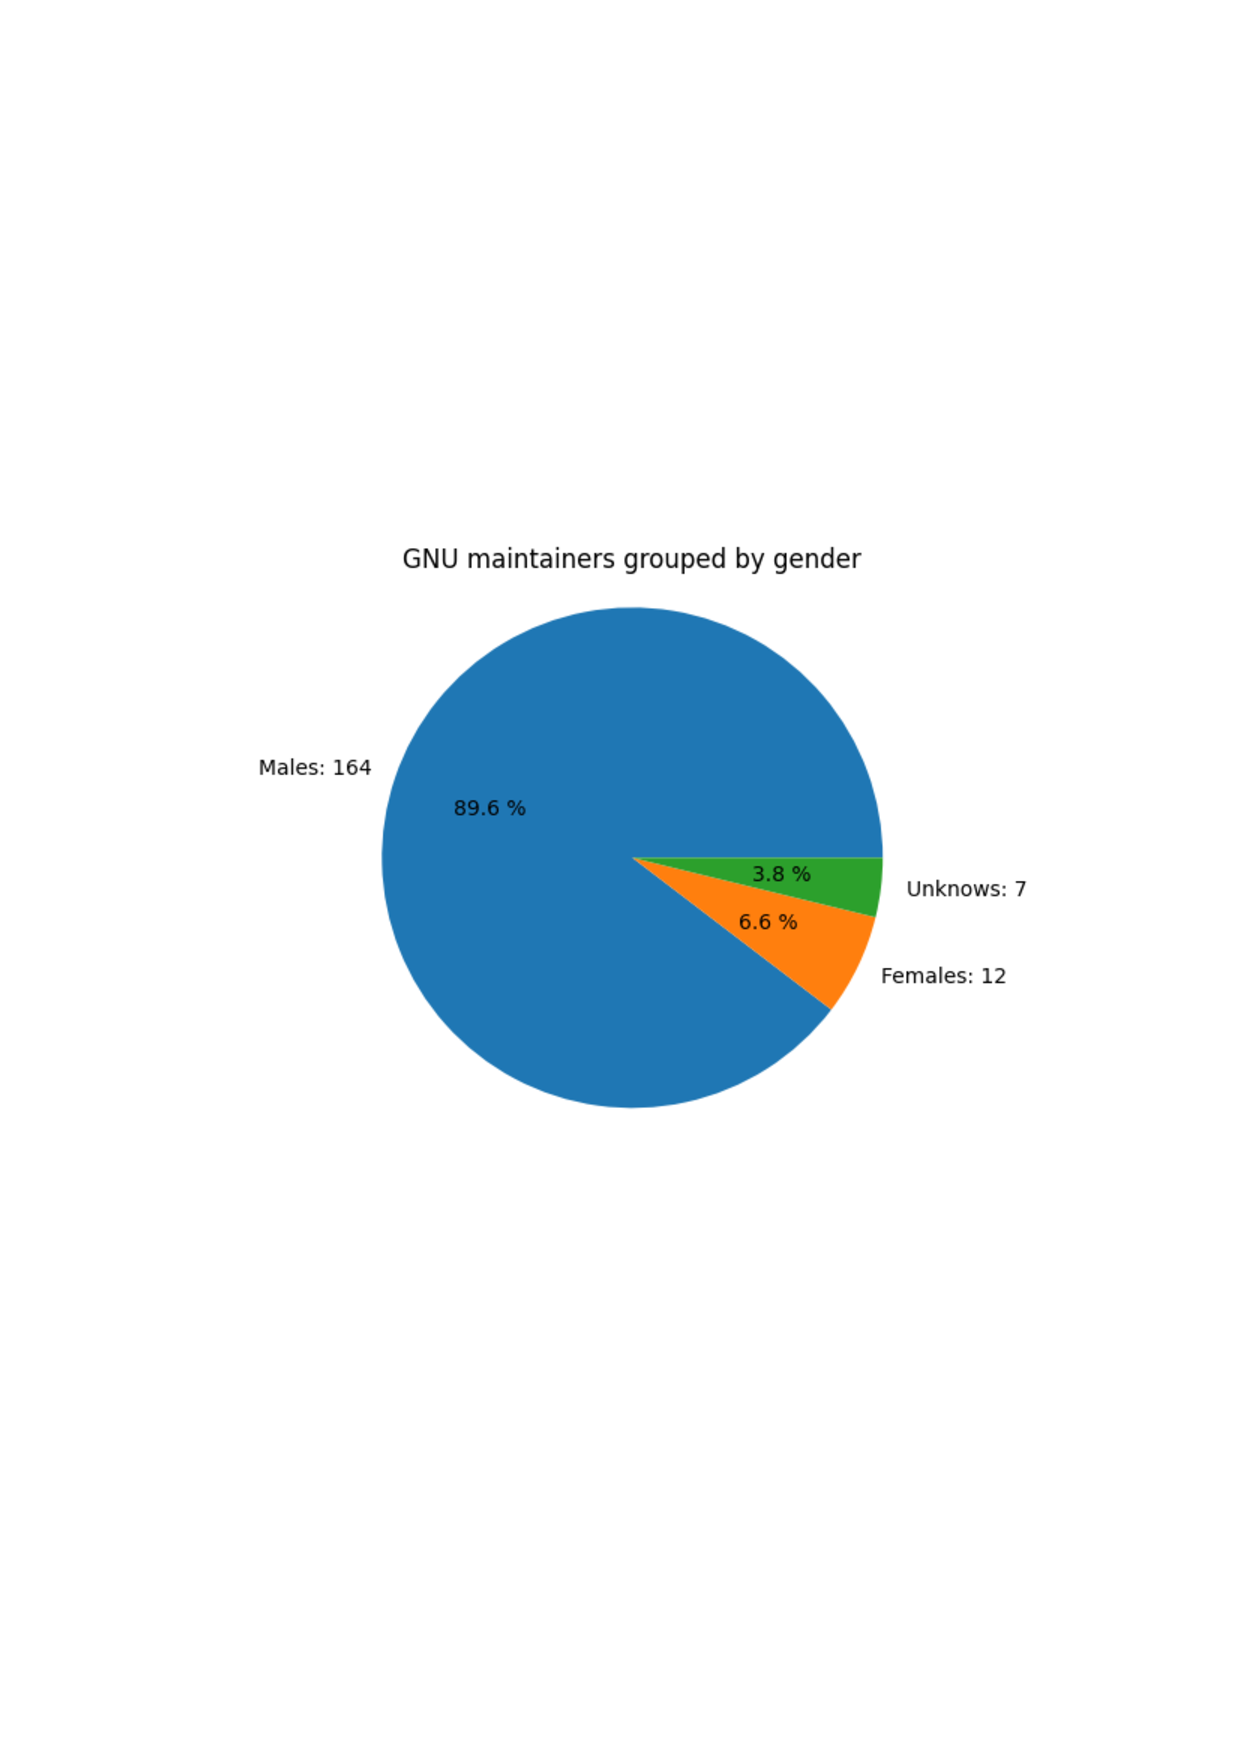
\includegraphics[width=0.6\textwidth]{images/gnu-maintainers.gender.pdf}

GNU divides the developers in 164 males (89.6\%), 12 females (6.6\%)
and 7 unknows (3.8\%)

The GNU people has a number lowest in females, they are the founder of
the Free Software philosophy, the Debian principles and the Open
Source philosophy was invented later influenced by GNU with very
similar practical decisions (for example: deciding licenses for the
software). Richard Stallman returned to be president recently
apologizing by his personal behaviour with the
females.\footnote{https://www.fsf.org/news/rms-addresses-the-free-software-community}

%% These data reveals that the situation has been improved with respect
%% the long time. In \cite{10.1007/978-3-319-39225-7_13} speaks about a
%% female participation of around 2 {\%} to 5 {\%}.

\section{Datasets}
\label{sec:datasets}

Name-to-gender inference services and tools apply several methods for estimating the gender from a given name. 
As a starting point, however, all of them rely on a dataset that contains information on what gender a name usually can be attributed to.

There are several sources to create these databases, being the most common:  
(1) a census published with a free license (open census way), 
(2) a dataset released with a free license in a free software package (free software way), 
(3) a dataset retrieved from commercial APIs (commercial API way), and
(4) a dataset which is the result of an investigation and that has been released publicly (scientific way).

In \texttt{damegender}, we are including Open Data census about names and gender, usually offered by governments, such as the ones from Spain (by means of INE.es, the Spanish National Statistics Institute), Uruguay, USA and UK. 
%The datasets provided by the software package is incrementing the speed retrieving data.

\begin{table*}[ht]
\footnotesize
\begin{tabular}[]{lcccccc}
\hline
Service / Tool $->$ & Gender API & gender-guesser & genderize.io & NameAPI & NamSor & damegender\tabularnewline
\hline
Database size & 431M & 45K & 114M & 1M & 4G & 57K \tabularnewline
Regular data updates & Yes & no & No & Yes & Yes & Yes\tabularnewline
Unstructured full name strings & Yes & No & No & Yes & No & Yes\tabularnewline
Surnames & Yes & No & No & Yes & Yes & Yes\tabularnewline
Non-Latin alphabets & Partial & No & Partial & Yes & Yes & No\tabularnewline
Implicit geo-localization & Yes & No & No & Yes & Yes & No\tabularnewline
Exists locale & Yes & Yes & Yes & Yes & Yes & Yes\tabularnewline
Assignment type & P & B & P & P & P & P \tabularnewline
Free parameters & T,P & G & P,C & T & S & T,C\tabularnewline
Prediction & No & No & No & No & No & Yes\tabularnewline
Free license & No & Yes & No & No & No & Yes\tabularnewline
REST API & Yes & No & Yes & Yes & Yes & Planned\tabularnewline
Limits number of requests & Yes (200) & \infinity & Yes & Yes & Yes & \infinity \tabularnewline
Subscription (100K requests/month)	 & 79 & 0 & 7 & 150 & 80 & 0 \tabularnewline
\hline
\end{tabular}
\caption{Comparison of the different features that name-to-gender inference services and tools offer. Assignment type = \{P: Probabilistic; B: Binary\}. Free Parameters = \{T: total\_names; P: probability; C: count; G: gender; T: trust; S: scale \}. The subscription price is given in euro.}
\vspace{0.3cm}
\label{table:comparison}
\end{table*}


Some Open Datasets, such the one offered by INE.es or the government of the US offer support for surnames and how they are related to ethnicity. 
In particular, the dataset from the government of the US offers a probability of the race, and the Spanish INE.es gives the number of people with a surname with a nationality different to the Spanish nationality.

Generally, a name has a strong weight to determine if it is a male or a female using this procedure.
For instance, David is registered 365,196 times as male, but 0 times as female in the data offered by the Spain National Institute of Statistics.
There are names that heavily depend on the region. 
For instance, Andrea would be considered a female name in Germany, but a male name in Italy.
Hence, we are using the census approach as base of truth to distinguish if a name is male or female in a geographical area. 
However, many countries do not provide Open Data census about gender and names, although our hope is that they will do in the near future.

%From the scientific point of view, the value of using Open Data is to allow that the experiment can be reviewed by peers on an automatic and legal way (using proprietary data the reviewer should request it separately to make the review).

%This approach is valid, but it consumes many time and efforts, although could be useful if there not a legal way to build the dataset.

We have evaluated to include data from the second option (datasets released with a free license). 
For instance, the Natural Language Tool Kit offers 8,000 labeled English names classified as male or female. 
Another example is \texttt{Gender Guesser}, which provides a good dataset for international names with different categories to define the probability. 
Although these datasets can be incorporated into \texttt{damegender}, the problem with them is that, in general, we have observed that they do not have the quality of National Statistics Institutes. 

%This approach is similar to use a dataset released with a paper in a journal, the advantage is to understand and add new names with a solid criteria accepted by the scientific community.

The third approach is to create the dataset from existing, usually commercial solutions.
Here we have to trust their results, in the same way we trust search engines when we make searches in Internet.
This is because commercial APIs can be seen as a black box -- we do not know where the data comes from and how it has been treated.
But, at least, we can measure its quality, as we will do next.
So, we will see that --at this point-- commercial APIs offer better results than other solutions.
That is why \texttt{damegender} gives the possibility to include data from them.
It is possible to download JSON files from the main commercial name-to-gender inference API solutions (e.g., \texttt{genderapi}, \texttt{genderize}, \texttt{namsor}, \texttt{nameapi}) and use it as the dataset.
There are certain uses that are currently only available in such tools.

% One user can build proprietary datasets on this way using an average weighted by the precision or accuracy of each Application Programming Interface measured with \texttt{damegender} with an open dataset as base of truth.




\section{Feature comparison with other tools}
\label{sec:comparison}

Standard commercial name-to-gender inference APIs usually guess the gender for a single name or a list of names (from a CSV file or an API call). 
To express geolocalization the user can also give surnames, a country ISO code, or specify a language.
Generally, you can give a probability and a counter associated to a name and gender in a certain population.


The features observed in this framework are: (i) database size (as of January 2018), (ii) if there are regular data updates, (iii) if they handle unstructured full name strings, (iv) if they handle surnames, (v) if they handle non-Latin alphabets, (vi) if implicit geolocalization is available, (vii) if locale exists, (viii) the type of assignment, (ix) if free parameters are possible, (x) if they offer prediction, (xi) if the tool is released under an open source license, (xii) if they offer an API, (xiii) the amount of monthly free requests, and (xiv) the monthly subscription cost (calculated for 100,000 requests/month)).

We have used this comparison framework and have updated it to the current situation and extended it with \texttt{damegender}.
Results can be found in Table~\ref{table:comparison}.
As it can be observed, commercial services have the advantage of owning large datasets, in the order of millions or even of billions of entries.
The most advanced ones offer support for non-Latin alphabets.
However, they limit the amount of free requests that can be performed and their costs range from 7 euro to 150 euro per month.

\section{Reproducing values of accuracy and confusion matrix}
\label{sec:reproducing}

%\begin{table*}[]{@{}lllllll@{}}
\begin{table}[t]
\footnotesize
\begin{tabular}[]{lcccc}
  \hline
  API & Acc & Prec & F1 & Recall\tabularnewline
\hline
Genderapi & 0.969 & 0.972 & 0.964 & 1.0\tabularnewline
Genderize & 0.927 & 0.976 & 0.966 & 1.0\tabularnewline
Damegender (SVC)\footnote{SVC is the acronym of Support Vector Classification, the Machine Learning algorithm that Damegender was using with this results} & 0.879 & 0.972 & 0.972 & 1.0\tabularnewline
Namsor & 0.867 & 0.973 & 0.924 & 1.0\tabularnewline
Nameapi & 0.830 & 0.974 & 0.905 & 1.0\tabularnewline
Gender Guesser & 0.774 & 0.985 & 0.872 & 1.0\tabularnewline
\hline
\end{tabular}
\caption{Comparison of measures of the quality of the results for the tools under study.}
\label{table:DifferentAccuraciesMeasures}
\end{table}

In this section, we will analyze the quality of the service of existing name-to-gender inference services and tools.
There are different ways to express the probability of a successful identification (e.g., confidence, scale, accuracy, precision, and recall).
We can also inspect the confusion matrix to understand where the tools and services succeed or fail, and to analyze the different errors measures (error coded, error coded without not applicable values, error gender bias, not applicable coded) that can happen.



In their dataset, gender is classified as male, female, or unknown. 
We have used this dataset, not considering the unknown variable, for our experiments.

The results, using common information retrieval metrics, can be seen in Table~\ref{table:DifferentAccuraciesMeasures}.
Accuracy is the ratio of correctly predicted observation to the total observations.
It should be noted that \emph{Accuracy} can be a misleading metric for imbalanced data sets.
This is because for a sample with 85 negative and 15 positive values, classifying all values as negative would give an accuracy score of 0.85.
In those cases, it is better to report other measures, such as the balanced accuracy, which normalizes true positive and true negative predictions by the number of positive and negative samples.
As Santamaría and Mihaljevi\'c's data does not come from the IT domain, we can use accuracy in our research.
Precision is the fraction of relevant instances among the retrieved instances.
Recall is the fraction of the total amount of relevant instances that were actually retrieved.
In our case, we have left no name out, so recall is 1 for all tools.
Precision and recall are sometimes used together in the F1 Score (or f-measure) to provide a single measurement for a system.
As can be observed, \texttt{Genderapi} and \texttt{Genderize} obtain the best results -- although all solutions are close and reach results better than 0.8 for accuracy, except for \texttt{Gender Guesser}.
\texttt{damegender} offers relatively good results.
Given, however, that its focus is mainly to be used in the IT domain, where the gender is highly imbalanced, we are very positive about its precision, as accuracy is not that relevant as noted above.

%\grex{Deberiamos explicar que es cada una de las metricas. Y tambien por que tenemos 1.0 de recall en todos los casos.}
%\davidam{Esto es un poco largo de explicar. Está explicado de una manera abreviada más arriba. Si te ves con energías para explicarlo, está explicado en https://easychair.org/publications/preprint/vthL}



\begin{table}[t]
\footnotesize
\begin{tabular}[]{lrrrr}
  \hline
  APIs          & gender & male & female & undef \tabularnewline
\hline
%%\endhead
Genderapi         & male    & 3589 & 155  &  67 \tabularnewline
                  & female  & 211  & 1734 &  23 \tabularnewline
Damegender       & male    & 3663 & 147  &   0 \tabularnewline
                & female  & 551  & 1497 &   0 \tabularnewline
Genderguesser     & male    & 3326 &  139 & 346 \tabularnewline
                  & female  & 78   & 1686 & 204 \tabularnewline
Namsor            & male    & 3325 & 139  & 346 \tabularnewline
                  & female  & 78   & 1686 & 204 \tabularnewline
Genderize         & male    & 3157 & 242  & 412 \tabularnewline
                  & female  & 75   & 1742 & 151 \tabularnewline
Nameapi           & male    & 2627 & 674  & 507 \tabularnewline
                  & female  & 667  & 1061 & 240 \tabularnewline 
\hline
\end{tabular}
\caption{Confusion matrix tables by APIs}
\label{table:ConfusionMatrixTables}
\end{table}


We have performed a comparison using a confusion matrix for the software/tools under study (see Table~\ref{table:ConfusionMatrixTables}).
The most important tools (\texttt{Namsor}, \texttt{Genderapi}, and \texttt{Genderize}) improve the values of accuracy with respect to the previous comparison.
In particular, \texttt{Genderapi} improves the results for \emph{undefined}.
For \texttt{Genderize}, we obtain exactly the same results. 
For \texttt{Genderguesser}, however, we obtain different results, which is to some extent not expected, because the software has not been modified for several years.
\texttt{Nameapi}'s results is changing from male to female with more errors. 
In \texttt{Namsor}, the results are similar. 
\texttt{damegender} is not guessing undefined because we predict with machine learning (using an SVC algorithm) if the string is not in the database.

\begin{table*}
\footnotesize
\center
\begin{tabular}[]{lrrrr}
\hline
API & error & error w/o na & na coded & error gender bias\tabularnewline
\hline
%\endhead
Damegender (SVC)\footnotemark[1] & 0.121 & 0.121 & 0.0 & -0.07\tabularnewline
GenderApi & 0.167 & 0.167 & 0.0 & -0.167\tabularnewline
Gender Guesser & 0.225 & 0.027 & 0.204 & 0.003\tabularnewline
Genderize & 0.276 & 0.261 & 0.0204 & -0.0084 \tabularnewline 
Namsor & 0.332 & 0.262 & 0.095 & 0.01 \tabularnewline
Nameapi & 0.361 & 0.267 & 0.129 & 0.001 \tabularnewline
\hline
\end{tabular}
\caption{APIs and Errors}
\vspace{0.3cm}
\label{table:ApisAndErrors}
\end{table*}


In Table~\ref{table:ApisAndErrors} we can see the different measures for errors in the APIs.
\emph{Error coded} defines if the true is different than the guessed one. 
\emph{Error coded without na} defines if the true is different than the guessed one, but without undefined results.
\emph{Error gender bias} allows to understand if the error is bigger for guessing males than females or viceversa.
The \emph{weighted error} defines if the true value is different than the guessed one, but giving a weight to the guessed as undefined.
The most relevant information is a high index of errors for \texttt{Nameapi} and \texttt{Namsor},
while \texttt{GenderApi} and \texttt{damegender} have a low index of errors.


\section{Machine Learning}
\label{sec:ml}

\subsection{Comparing ML algorithms}

\begin{table}
\footnotesize
\center
\begin{tabular}[]{lcccc}
  \hline
  ML Algorithm & Acc & Prec & F1 & Recall \tabularnewline
  \hline
  %\endhead
 Support Vector Machines             &    0.879 &     0.972 &   0.972 &    1.0  \tabularnewline
 Random Forest                       &    0.862 &     0.902 &   0.902 &    1.0  \tabularnewline
 NLTK (Bayes)                        &    0.862 &     0.902 &   0.902 &    1.0  \tabularnewline
 Multinomial Naive Bayes             &    0.782 &     0.791 &   0.791 &    1.0  \tabularnewline
 Tree                                &    0.764 &     0.821 &   0.796 &    1.0  \tabularnewline
 Stoch. Gradient Distrib.            &    0.709 &     0.943 &   0.815 &    1.0  \tabularnewline
 Gaussian Naive Bayes                &    0.709 &     0.968 &   0.887 &    1.0  \tabularnewline
 Bernoulli Naive Bayes               &    0.699 &     0.965 &   0.816 &    1.0  \tabularnewline
\hline
\end{tabular}
\caption{Machine Learning Algorithms and accuracy measures}
\label{table:MLAccuracies}
\end{table}

\begin{table*}
\footnotesize
\center
\begin{tabular}[]{lccccccc}
  \hline
Dataset & contains a & last is a & last is o & last is consonant & last is vowel & 1st is consonant & 1st is vowel  \tabularnewline
  \hline
  %\endhead
 Uruguay (F) &    0.816 &         0.456 &         0.007 &                 0.287 &             0.712 &                  0.823 &              0.177  \tabularnewline
 Uruguay (M) &    0.643 &         0.249 &         0.062 &                 0.766 &             0.234 &                  0.771 &              0.228  \tabularnewline
 Spain (F)   &    0.922 &         0.588 &          0.030 &                 0.271 &             0.728 &                  0.772 &              0.228  \tabularnewline
 Spain (M)   &    0.818 &          0.030 &         0.268 &                 0.569 &              0.430 &                  0.763 &              0.236  \tabularnewline
 UK (F)      &    0.825 &         0.374 &         0.013 &                 0.322 &             0.674 &                  0.765 &              0.235  \tabularnewline
 UK (M)      &    0.716 &         0.036 &         0.039 &                  0.780 &             0.218 &                  0.799 &                0.200  \tabularnewline
 USA (F)     &    0.816 &         0.456 &         0.007 &                 0.287 &             0.712 &                  0.823 &              0.177  \tabularnewline
 USA (M)     &    0.643 &          0.020 &         0.061 &                 0.765 &             0.234 &                   0.840 &              0.159  \tabularnewline
 Canada (F)  &    0.659 &         0.189 &         0.005 &                 0.591 &             0.408 &                  0.838 &              0.160  \tabularnewline
 Canada (M)  &    0.752 &          0.220 &         0.025 &                  0.540 &             0.456 &                  0.818 &              0.181  \tabularnewline
Australia (F)      &    0.922 &         0.588 &         0.033 &                 0.272 &             0.728 &                  0.772 &              0.228 \tabularnewline
 Australia (M)        &    0.818 &          0.030 &         0.269 &                  0.570 &              0.430 &                  0.763 &              0.237 \tabularnewline
 
\hline
\end{tabular}
\caption{Informative features for different countries. F stands for females, and M for males.}
\vspace{0.3cm}
\label{table:InfoFeatures}
\end{table*}


Table~\ref{table:MLAccuracies} shows the accuracy measures for some Machine Learning algorithms used in our guessing. 
The best results are given by Support Vector Machines and Random Forest -- with those algorithms \texttt{damegender} achieves values that are close to more mature, proprietary solutions.
It should be noted that as a result of using machine learning techniques, our classifier is binary (male and female), so no \emph{unknown} is given as output.

\subsection{Experimenting with some features}

We have developed some additional experimental functionality that allows to analyze our database according to some features using machine learning algorithms.
To test our approach, we have selected some features of names, such as a being the first letter, a (or o) being the last letter, contains the letter a, first letter is a vowel, last letter is a vowel, last letter is a consonant, or last letter is a. 
The selection of the features was verified with Principal Component Analysis.
The datasets used in this experiment were the ones from the National Institute of Statistics (Spain, Uruguay, United Kingdom, United States of America, Australia and Canada).
The most relevant results for the different datasets used are offered in Table~\ref{table:InfoFeatures}.

As expected, countries that share language offer similar results, i.e., the variation of the chosen features between males and females is comparable.
This is the case for Uruguay and Spain (Spanish), and USA and UK and Australia (English).
In Canada, a country that has an ample French-speaking community these features show a different trend.

For instance, the feature \emph{containing the letter a in the name} varies 0.2 from males to females for USA and Uruguay, and 0.1 from males to females for United Kingdom, Australia, and Spain.
The feature \emph{the last letter is an a} varies 0.5 from males to females for Australia and Spain, around 0.4 for USA and United Kingdom and 0.2 in
Uruguay.
The feature \emph{the last letter is an o} varies 0.2 in (Spain, Australia) from females to males and is equal in Uruguay, USA, United Kingdom.
For the feature \emph{the last letter is a consonant} all countries give as a result that males do have it more frequently, with results that range from 0.3 to 0.5: Uruguay and USA (0.5), United Kingdom (0.4), Australia and Spain (0.3). 
So, the feature \emph{the last letter is a vowel} is, as expected, the reverse of the feature \emph{the last letter is a consonant}. 
The features \emph{the first letter is a consonant} or \emph{the first letter is a vowel} are, however, non-significant as they offer similar results in English and Spanish.

We have done this experiment with the NLTK and INE.es datasets, with the values of accuracy reaching up to 0.745.
So it makes sense to expect better results in random datasets if we add new languages and countries.
However, our solution is not providing Arabic or Chinese alphabets, yet.
The results of this experiment could be used to provide a good solution for nicknames, diminutives, or similar.


\section{Limitations and further research}
\label{sec:limitations}

The market of gender detection tools and services is currently dominated by companies based on payment services through Application Programming Interfaces.
Without doubt, they offer good results, with high accuracy values.
However, their inner working cannot be studied (i.e., they work as a black-box for the outsider) and the fees that have to be paid for using their service are sometimes out of the reach of many researchers.
That is why we propose a new tool, called \texttt{damegender}, with the aim of having open data of name-to-gender inference, which offers more flexibility and where researchers can build on top of it.
This tool is offered under a free software license and is available on GitHub for download and enhancement.
As we have shown in this paper, although still incipient, the tool offers good accuracy values based on the use of public databases from government bodies and on the use of machine learning algorithms.
Nonetheless, we have to note that \texttt{damegender} is still under development, and that it has to be applied to several real repositories to confirm its benefits and address its limitations (such as a small database size of gendered names).

In addition, we have shown a glimpse of how several features of the names could be used to guess the gender if we do not have the real name, but nicknames or diminutives, a situation that is very common in free software development-supporting tools, such as IRC channels.
This experiment is at this point very preliminary, and we would like to work more on it.

All in all, we hope the \texttt{damegender} tool can become a cornerstone for the scientific advancement of the study of gender (including gender gap) and diversity in the IT, and in particular in the free software community.
We have therefore many hopes in linking the output of repositories like the ones that can be fetched by Perceval (git, mbox mailing lists, Gerrit, Bugzilla, etc.).
As a result, we envision a free and international dataset with support for all languages and cultures.


\section*{Acknowledgments}

We would like to thank: Lucía Santamaría and Helena Mihaljevi\'c for the previous work; Daniel Izquierdo and Laura Arjona for starting this research field at URJC; Jesus González Boticario and his team at UNED for the motivation towards machine learning; all those working with Jesus González Barahona and Gregorio Robles.

\bibliographystyle{alpha} 
\bibliography{uc3m}

\end{document}


